\section{Results}
% TODO: draft from the drafting sheet; every number as \N{key}

\subsection{Discrimination and Learning Curves}
% TODO: draft from the drafting sheet; every number as \N{key}

\subsection{Calibration}
% TODO: draft from the drafting sheet; every number as \N{key}

\subsection{Robustness to Missing Values and Noise}
% TODO: draft from the drafting sheet; every number as \N{key}

\subsection{Explanation Agreement}
% TODO: draft from the drafting sheet; every number as \N{key}

% Example environments (commented out until the figures/tables are used; the bundle
% checker verifies that every target below exists inside the bundle):
% \begin{figure*}[t]
%   \centering
%   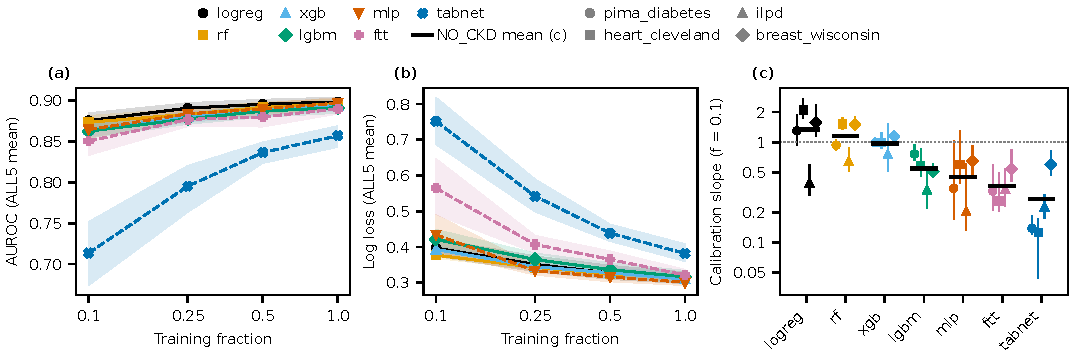
\includegraphics[width=\textwidth]{figures/fig_main_learning_calibration.pdf}
%   \caption{TODO: caption}
%   \label{fig:learning-calibration}
% \end{figure*}
% \begin{figure*}[t]
%   \centering
%   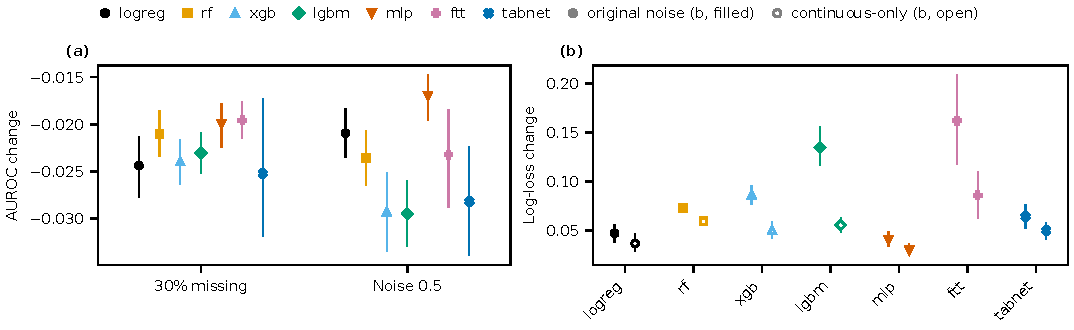
\includegraphics[width=\textwidth]{figures/fig_main_robustness.pdf}
%   \caption{TODO: caption}
%   \label{fig:robustness}
% \end{figure*}
% \begin{figure*}[t]
%   \centering
%   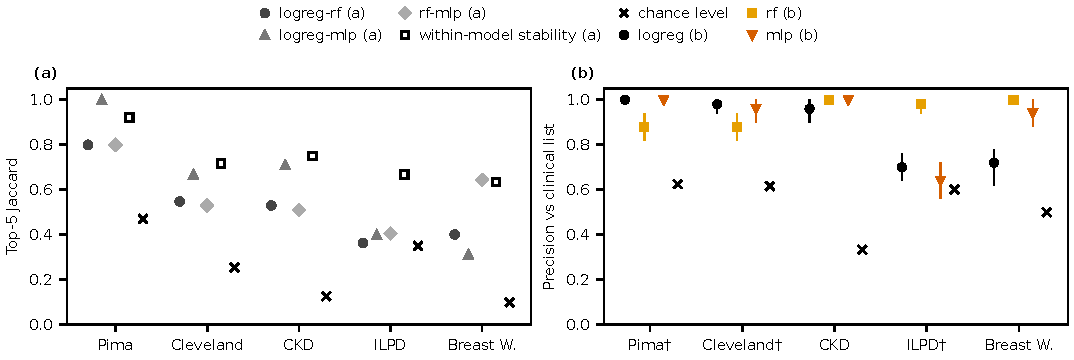
\includegraphics[width=\textwidth]{figures/fig_main_explanations.pdf}
%   \caption{TODO: caption (define the dagger: chance precision at least 0.60)}
%   \label{fig:explanations}
% \end{figure*}
% \begin{figure}[t]
%   \centering
%   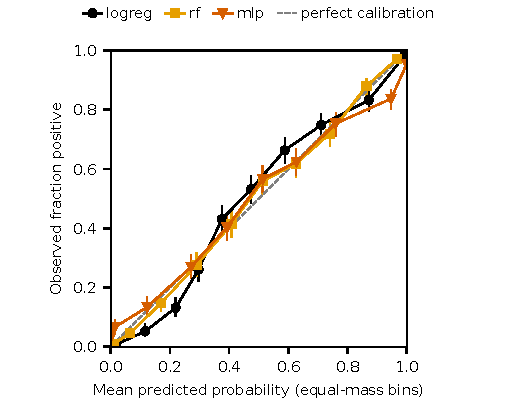
\includegraphics[width=\columnwidth]{figures/fig_main_reliability.pdf}
%   \caption{TODO: caption}
%   \label{fig:reliability}
% \end{figure}
% % Generated by scripts/make_paper_tables.py -- do not edit by hand.
% Every numeric cell is a numbers-book macro (keys in paper/evidence/numbers.json).
\begin{table*}[t]
\centering
\footnotesize
\caption{TODO: caption}
\label{tab:main}
\begin{tabular}{lccccccc}
\toprule
Model & \multicolumn{2}{c}{AUROC, $f{=}1.0$} & \multicolumn{2}{c}{AUROC, $f{=}0.1$} & \multicolumn{1}{c}{Log loss, $f{=}1.0$} & \multicolumn{1}{c}{Log loss, $f{=}0.1$} & \multicolumn{1}{c}{Slope, $f{=}0.1$} \\
\cmidrule(lr){2-3}\cmidrule(lr){4-5}\cmidrule(lr){6-6}\cmidrule(lr){7-7}\cmidrule(lr){8-8}
 & ALL5 & NO\_CKD & ALL5 & NO\_CKD & ALL5 & ALL5 & NO\_CKD \\
\midrule
LogReg & \textbf{\N{auroc-mean-logreg-all5-f1.0}} & \textbf{\N{auroc-mean-logreg-nockd-f1.0}} & \textbf{\N{auroc-mean-logreg-all5-f0.1}} & \textbf{\N{auroc-mean-logreg-nockd-f0.1}} & \N{logloss-mean-logreg-all5-f1.0} & \N{logloss-mean-logreg-all5-f0.1} & \N{slope-logreg-nockd-f0.1} \\
RF & \N{auroc-mean-rf-all5-f1.0} & \N{auroc-mean-rf-nockd-f1.0} & \N{auroc-mean-rf-all5-f0.1} & \N{auroc-mean-rf-nockd-f0.1} & \N{logloss-mean-rf-all5-f1.0} & \textbf{\N{logloss-mean-rf-all5-f0.1}} & \N{slope-rf-nockd-f0.1} \\
XGBoost & \N{auroc-mean-xgb-all5-f1.0} & \N{auroc-mean-xgb-nockd-f1.0} & \N{auroc-mean-xgb-all5-f0.1} & \N{auroc-mean-xgb-nockd-f0.1} & \N{logloss-mean-xgb-all5-f1.0} & \N{logloss-mean-xgb-all5-f0.1} & \textbf{\N{slope-xgb-nockd-f0.1}} \\
LightGBM & \N{auroc-mean-lgbm-all5-f1.0} & \N{auroc-mean-lgbm-nockd-f1.0} & \N{auroc-mean-lgbm-all5-f0.1} & \N{auroc-mean-lgbm-nockd-f0.1} & \N{logloss-mean-lgbm-all5-f1.0} & \N{logloss-mean-lgbm-all5-f0.1} & \N{slope-lgbm-nockd-f0.1} \\
MLP & \N{auroc-mean-mlp-all5-f1.0} & \N{auroc-mean-mlp-nockd-f1.0} & \N{auroc-mean-mlp-all5-f0.1} & \N{auroc-mean-mlp-nockd-f0.1} & \textbf{\N{logloss-mean-mlp-all5-f1.0}} & \N{logloss-mean-mlp-all5-f0.1} & \N{slope-mlp-nockd-f0.1} \\
FT-Transformer & \N{auroc-mean-ftt-all5-f1.0} & \N{auroc-mean-ftt-nockd-f1.0} & \N{auroc-mean-ftt-all5-f0.1} & \N{auroc-mean-ftt-nockd-f0.1} & \N{logloss-mean-ftt-all5-f1.0} & \N{logloss-mean-ftt-all5-f0.1} & \N{slope-ftt-nockd-f0.1} \\
TabNet & \N{auroc-mean-tabnet-all5-f1.0} & \N{auroc-mean-tabnet-nockd-f1.0} & \N{auroc-mean-tabnet-all5-f0.1} & \N{auroc-mean-tabnet-nockd-f0.1} & \N{logloss-mean-tabnet-all5-f1.0} & \N{logloss-mean-tabnet-all5-f0.1} & \N{slope-tabnet-nockd-f0.1} \\
\bottomrule
\end{tabular}
\end{table*}

